Circles $\mathcal{P}$ and $\mathcal{Q}$ have radii $1$ and $4$, respectively, and are externally tangent at point $A$. Point $B$ is on $\mathcal{P}$ and point $C$ is on $\mathcal{Q}$ so that line $BC$ is a common external tangent of the two circles. A line $\ell$ through $A$ intersects $\mathcal{P}$ again at $D$ and intersects $\mathcal{Q}$ again at $E$. Points $B$ and $C$ lie on the same side of $\ell$, and the areas of $\triangle DBA$ and $\triangle ACE$ are equal. This common area is $\frac{m}{n}$, where $m$ and $n$ are relatively prime positive integers. Find $m+n$.

\begin{center}
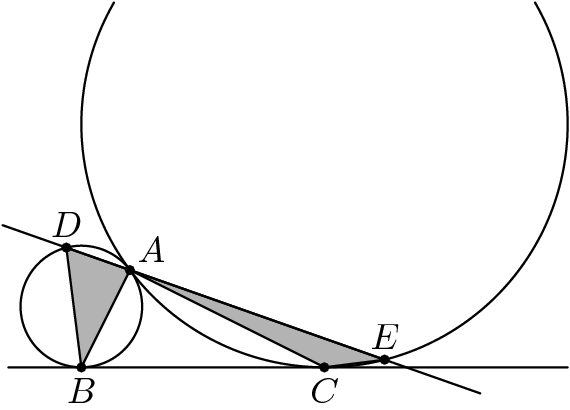
\includegraphics[width = 57.0mm]{img/fig0.png}
\end{center}